\section{Minimum Spanning Trees}
\begin{center}
    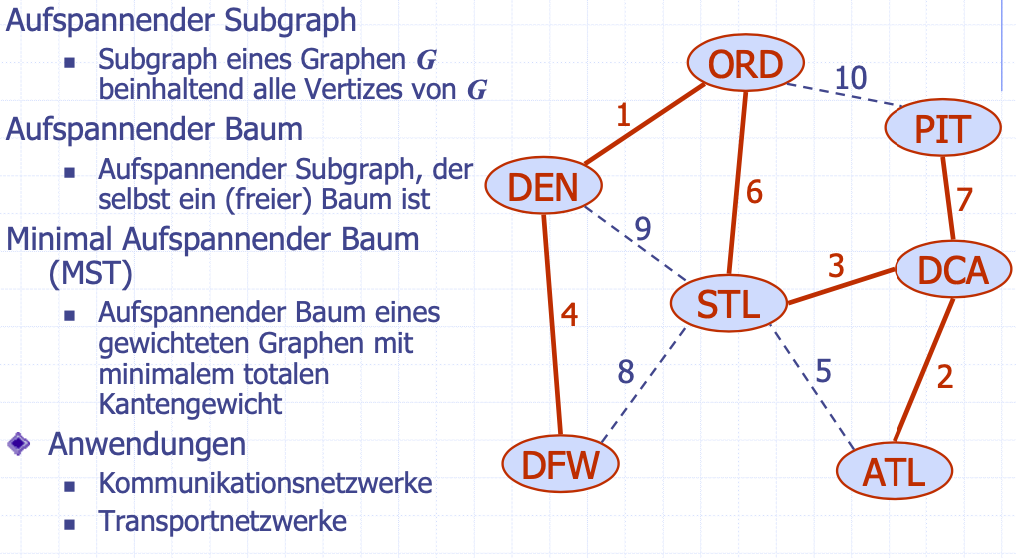
\includegraphics[scale=.32]{graphic/16 MinimumSpanningTrees/Minimum Spanning Tree.png}
\end{center}
\vspace{-8pt}

\subsection{Schlaufen-Eigenschaft}
\begin{center}
    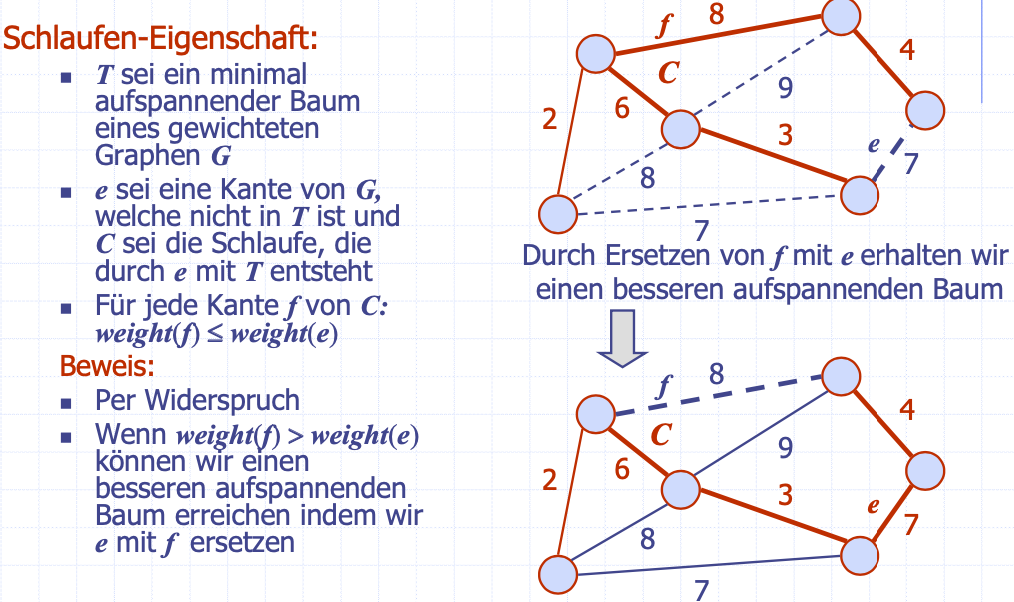
\includegraphics[scale=.32]{graphic/16 MinimumSpanningTrees/Schlaufen-Eigenschaft.png}
\end{center}
\vspace{-8pt}

\subsection{Aufteilungs-Eigenschaft}
\begin{center}
    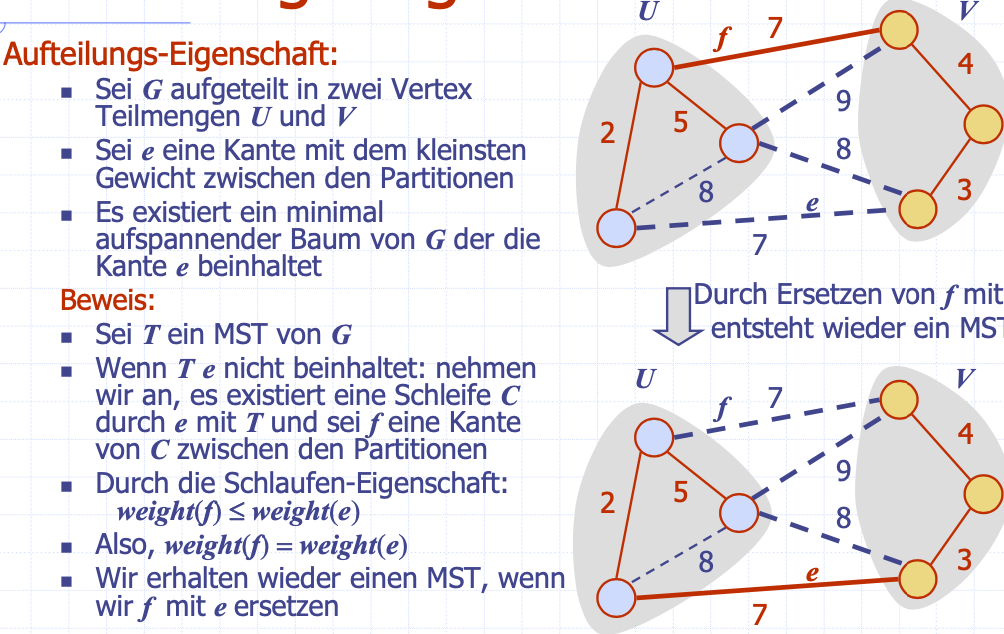
\includegraphics[scale=.32]{graphic/16 MinimumSpanningTrees/Aufteilungs-Eigenschaft.png}
\end{center}
\vspace{-8pt}

\subsection{Kruskal’s Algorithmus}
\subsubsection{Datenstruktur}
\begin{itemize}
    \item Der Algorithmus behält einen Wald von Bäumen
    \item Eine Kante ist akzeptiert, wenn sie verschiedene Bäume verbindet
    \item Wir brauchen eine Datenstruktur welche eine Partition verwaltet. Z.B. eine Sammlung von disjunkten Sets mit folgenden Operationen:
    \begin{itemize}
        \item find(u): Gibt ein Set U zurück enthaltend u
        \item union(u,v): ersetzt die Sets, welche u und v speichern mit deren Vereinigung
    \end{itemize}
\end{itemize}
\begin{center}
    \includegraphics[scale=.31]{graphic/16 MinimumSpanningTrees/Kruskal’s Algorithmus.png}
\end{center}
\vspace{-8pt}

\subsubsection{Repräsentation einer Partition}
\begin{itemize}
    \item Jedes Set ist in einer Sequenz gespeichert
    \item Jedes Element hat eine Referenz zurück auf das Set
    \begin{itemize}
        \item Operation find(u) benötigt O(1) Zeit und gibt das Set zurück, in dem u ist
        \item In der Operation union(u,v) verschieben wir die Elemente des kleineren Sets in die Sequenz des grösseren Sets und aktualisieren deren Referenzen
        \item Die Zeit für die Operation union(u,v) ist min($n_u,n_v$), wobei $n_u$ und $n_v$ die Grössen der Sets sind, die u und v beinhalten
    \end{itemize}
    \item Wenn ein Element verarbeitet wird, geht es in ein Set mit mindestens doppelter Grösse. Jedes Element wird also höchstens log n mal verarbeitet
\end{itemize}
\begin{center}
    \includegraphics[scale=.6]{graphic/16 MinimumSpanningTrees/Repräsentation einer Partition.png}
\end{center}
\vspace{-8pt}
\subsubsection{Partition-Basierte Implementation}
Eine partition-basierte Version von Kruskal’s Algorithmus führt Wolken-Vereinigungen mit union’s und Tests mit find’s aus
\begin{center}
    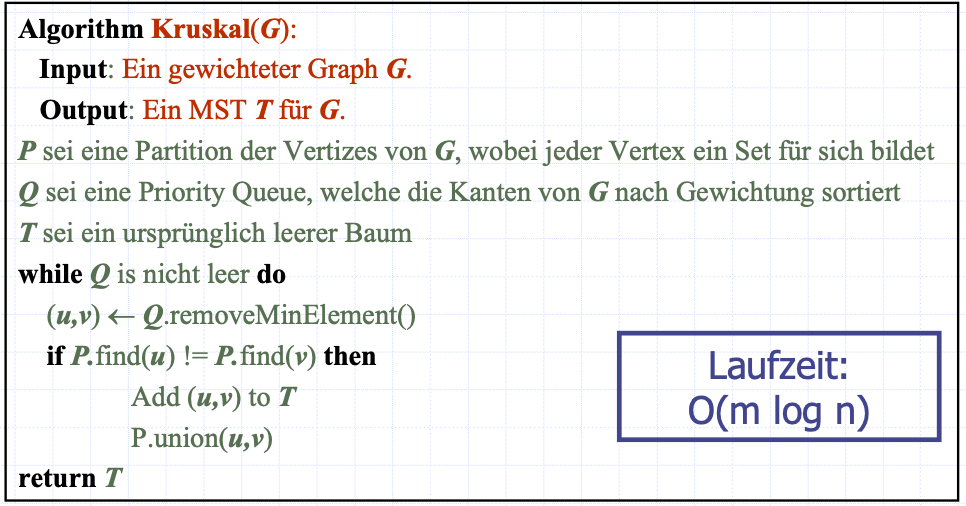
\includegraphics[scale=.35]{graphic/16 MinimumSpanningTrees/Partition-Basierte Implementation.png}
\end{center}
\vspace{-8pt}


\subsubsection{Beispiel}
\begin{center}
    \includegraphics[scale=.3]{graphic/16 MinimumSpanningTrees/Kruskal’s Beispiel.png}
\end{center}
\vspace{-8pt}

\subsection{Prim-Jarnik’s Algorithmus}
\begin{itemize}
    \item Gleich wie Dijkstra’s Algorithmus (für einen verbundenen Graphen)
    \item Wir nehmen einen beliebigen Vertex s und generieren den MST als eine Wolke von Vertizes von s
    \item Wir speichern zu jedem Vertex ein Label d(v) = die kleinste Gewichtung einer Kante, welche v mit einem Vertex der Wolke verbindet
    \item Bei jedem Schritt:
    \begin{itemize}
        \item Fügen wir der Wolke den Vertex u von ausserhalb der Wolke mit dem kleinsten Distanz-Label hinzu
        \item Wir aktualisieren die Labels der Nachbar-Vertizes von u
    \end{itemize}
\end{itemize}
\subsubsection{Laufzeit}
\begin{itemize}
    \item Methode incidentEdges wird für jeden Vertex einmal aufgerufen
    \item Wir setzen/lesen das Distanz-, Parent- und Locator-Label eines Vertex z insgesamt O(deg(z)) mal
    \item Setzen/Lesen eines Labels benötigt O(1) Zeit
    \item Jeder Vertex wird einmal in die Priority Queue eingefügt und einmal gelöscht, wobei jedes Einfügen oder Löschen O(log n) Zeit benötigt
    \item Der Schlüssel eines Vertex w in der Priority Queue wird maximal deg(w) mal geändert, wobei jede Änderung O(log n) Zeit benötigt
    \item Prim-Jarnik’s Algorithmus läuft in O((n + m) log n) Zeit, vorausgesetzt dass der Graph ist mit einer Adjazenz-Listen Struktur implementiert ist
\end{itemize}
\subsubsection{Algorithmus}
\begin{center}
    \includegraphics[scale=.35]{graphic/16 MinimumSpanningTrees/Prim-Jarnik’s Algorithmus.png}
\end{center}
\vspace{-8pt}

\subsubsection{Beispiel}
\begin{center}
    \includegraphics[scale=.3]{graphic/16 MinimumSpanningTrees/Prim-Jarnik’s bsp.png}
\end{center}
\vspace{-8pt}

\subsection{Boruvka’s Algorithmus}
\begin{center}
    \includegraphics[scale=.3]{graphic/16 MinimumSpanningTrees/Boruvka’s Algorithmus.png}
\end{center}
\vspace{-8pt}
\subsubsection{Beispiel}
\begin{center}
    \includegraphics[scale=.33]{graphic/16 MinimumSpanningTrees/Boruvka’s Algorithmus bsp.png}
\end{center}
\vspace{-8pt}


\paragraph{MST}
\begin{center}
    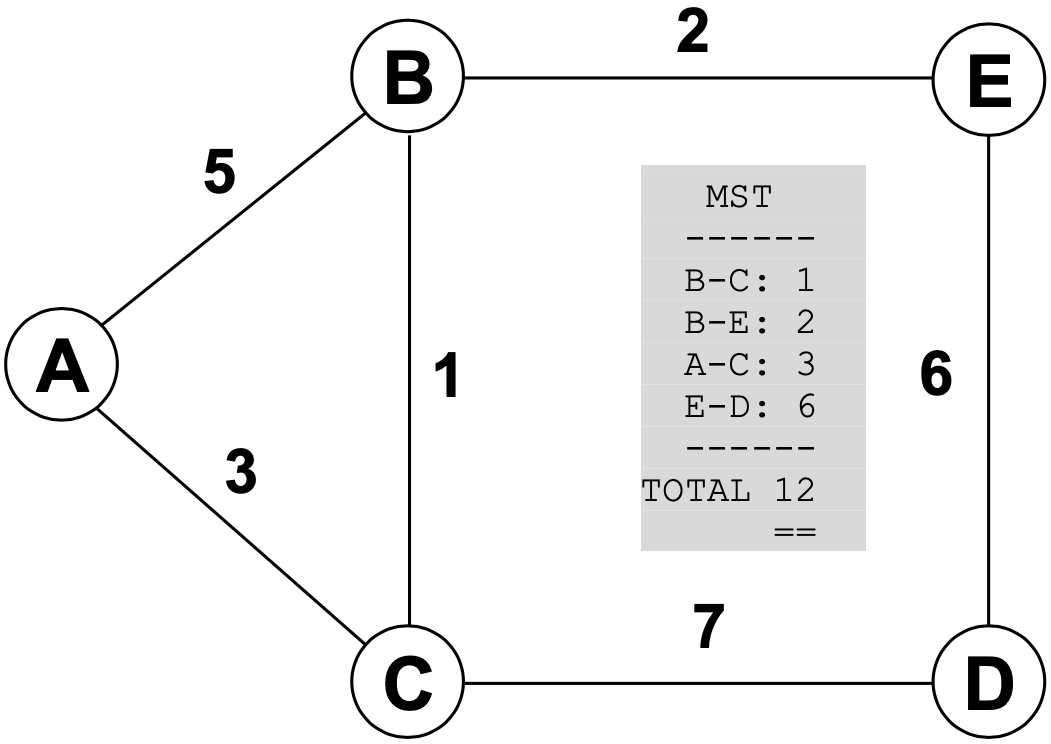
\includegraphics[scale=.3]{16 MinimumSpanningTrees/mst.png}
\end{center}

\paragraph{MST}
\begin{center}
    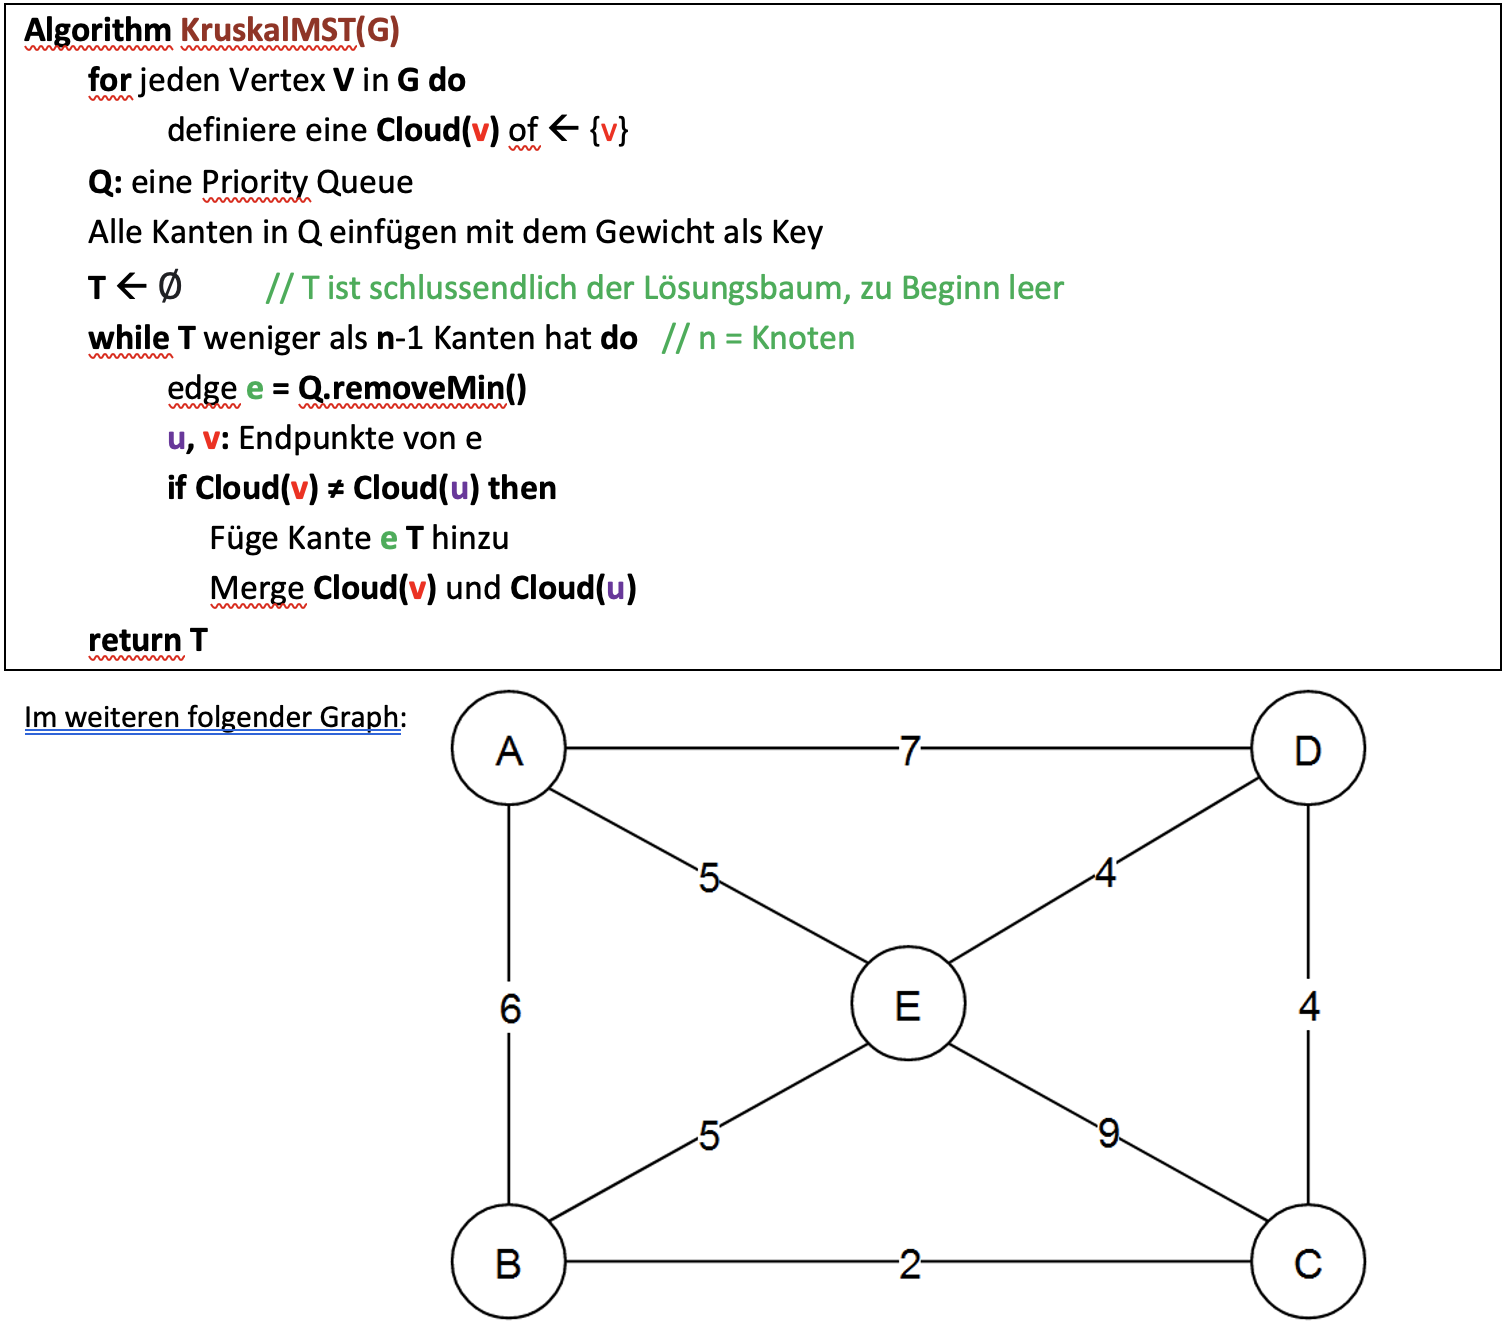
\includegraphics[scale=.2]{16 MinimumSpanningTrees/krusal1.png}
    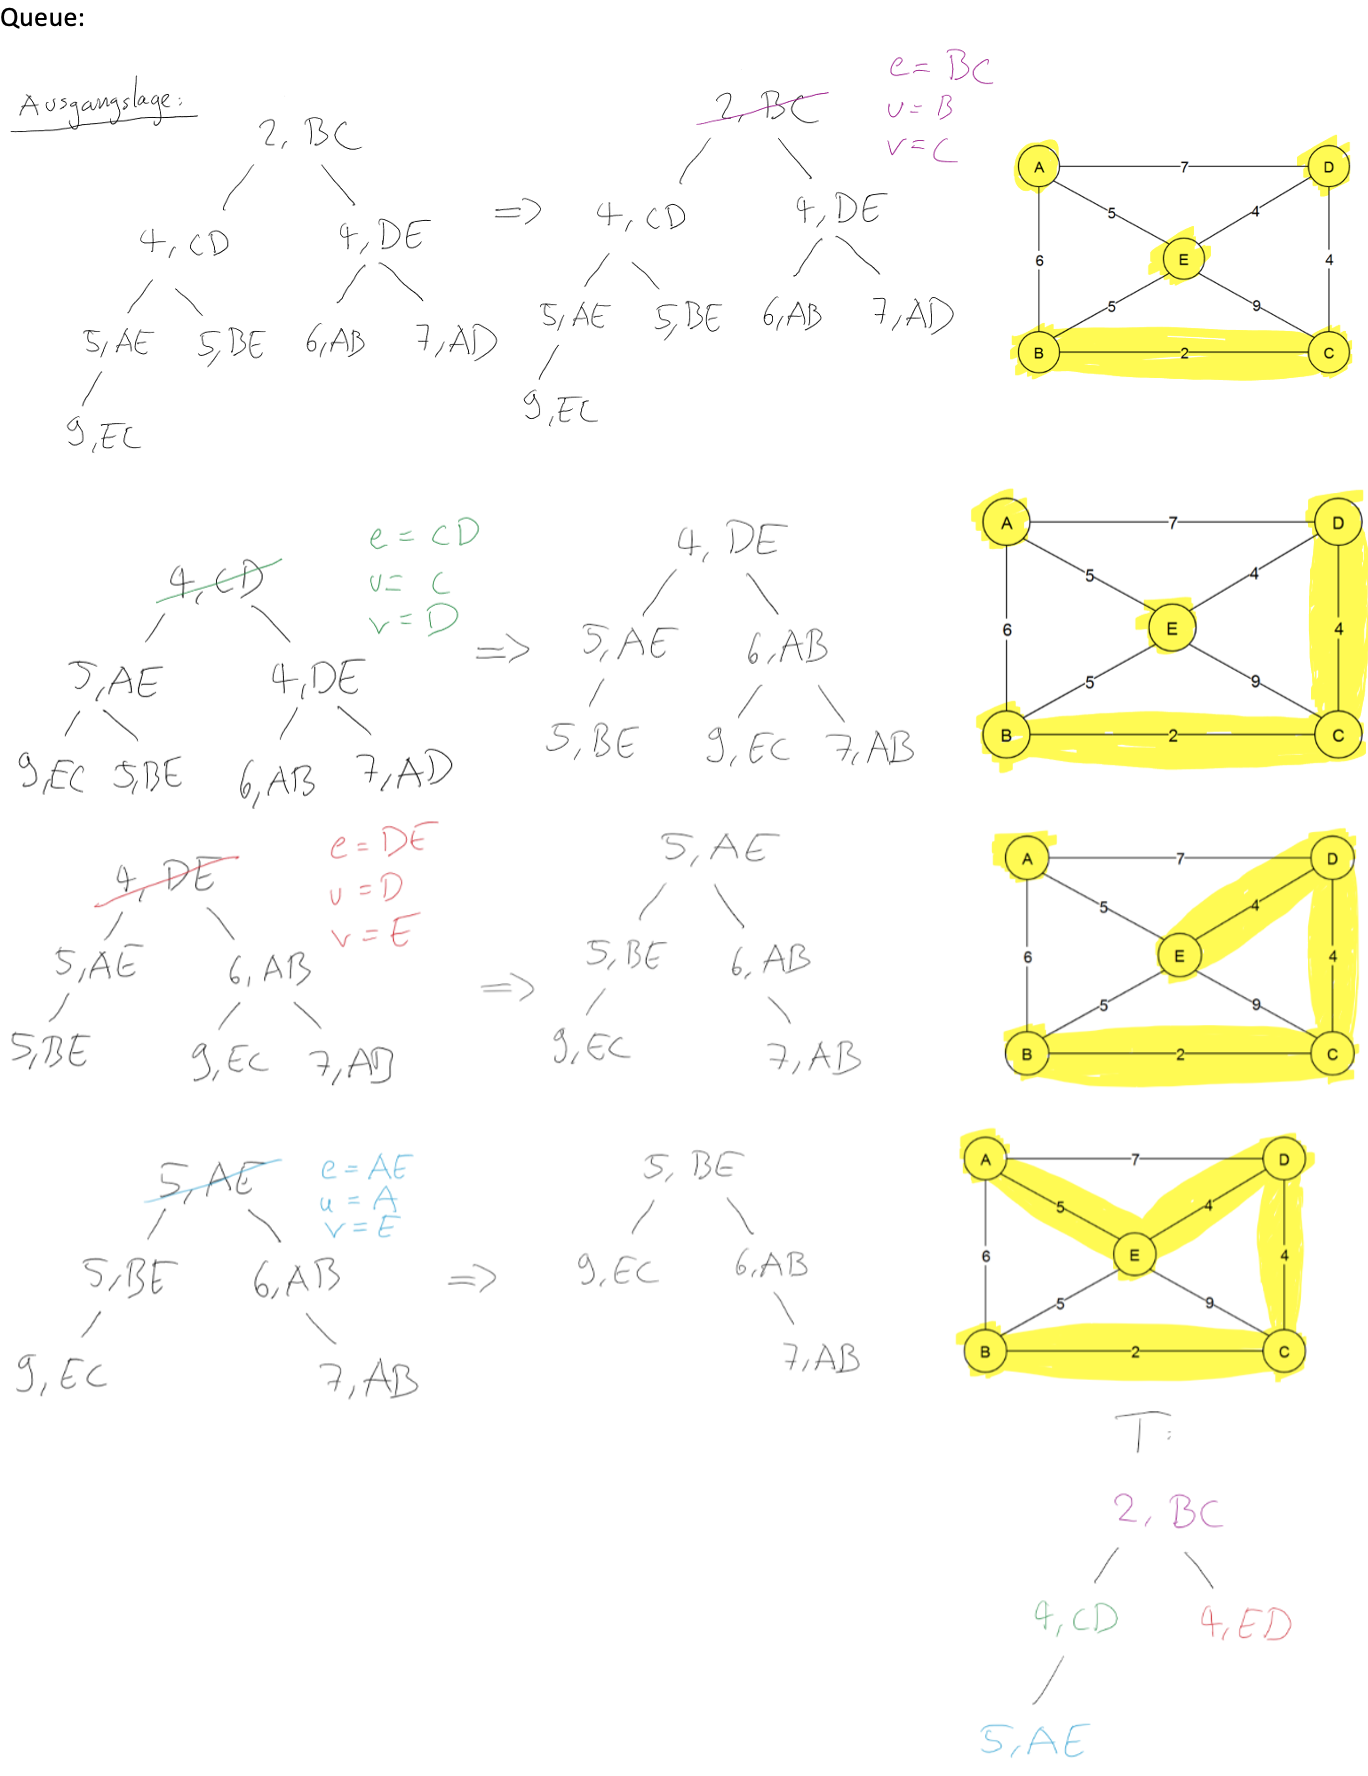
\includegraphics[scale=.26]{16 MinimumSpanningTrees/krusal2.png}
\end{center}



\newpage